% ============================================================
% 6. Fallos y tolerancia a fallos en RabbitMQ (Zambrano)
% ============================================================
\section{Fallos y tolerancia a fallos}

\begin{frame}{Riesgos de la concurrencia}
  \begin{itemize}
    \item \textbf{Condición de carrera:} dos trabajadores leen el mismo pedido y los dos lo despachan.
    \item \textbf{Bloqueo:} un trabajador espera a otro que nunca termina y la cola deja de avanzar.
    \item \textbf{Coordinación:} quién toma cada tarea y qué pasa si nadie confirma que la terminó.
  \end{itemize}
  \vspace{0.4cm}
  RabbitMQ entrega cada mensaje de una cola a un solo consumidor a la vez, pero eso no basta si el trabajador falla a mitad del proceso.
\end{frame}

\begin{frame}{Un trabajador falla con el pedido en la mano}
  \begin{enumerate}
    \item La cola entrega el pedido 125 al trabajador 1.
    \item El trabajador 1 se cae antes de terminar.
    \item Como nunca envió la confirmación (\texttt{ack}), RabbitMQ devuelve el pedido a la cola.
    \item El trabajador 2 lo recibe marcado como reentregado (\texttt{redelivered}) y lo procesa.
  \end{enumerate}
  \vspace{0.3cm}
  Si la confirmación fuera automática, el pedido se daría por entregado al salir de la cola y se perdería \cite{rabbitmq2026confirms}.
\end{frame}

\begin{frame}{Mecanismos de RabbitMQ}
  \begin{tabularx}{\textwidth}{lX}
    \toprule
    Mecanismo & Para qué sirve \\
    \midrule
    \texttt{ack} manual & El mensaje sale de la cola solo cuando el trabajador termina. \\
    \texttt{nack} / reencolar & El trabajador avisa que no pudo y el mensaje vuelve a la cola. \\
    Prefetch & Limita cuántos mensajes sin confirmar tiene cada trabajador. \\
    Publisher confirms & El broker le confirma al productor que guardó el mensaje. \\
    \bottomrule
  \end{tabularx}
  \vspace{0.3cm}
  {\small Fuente: \cite{rabbitmq2026confirms}}
\end{frame}

\begin{frame}{Incidente real: Kodus, enero de 2026}
  \begin{itemize}
    \item Migraron de un monolito a tres servicios conectados por RabbitMQ: Webhooks, API y Workers.
    \item 4 de enero: termina la migración.
    \item Días después: las revisiones de código se vuelven lentas y las máquinas se caen con carga.
    \item 23 de enero: encuentran la causa, con unos 900 \textit{pull requests} en cola.
  \end{itemize}
  \vspace{0.3cm}
  {\small Fuente: post-mortem oficial de Kodus \cite{malinosqui2026kodus}}
\end{frame}

\begin{frame}{Causas raíz del incidente de Kodus}
  \centering
  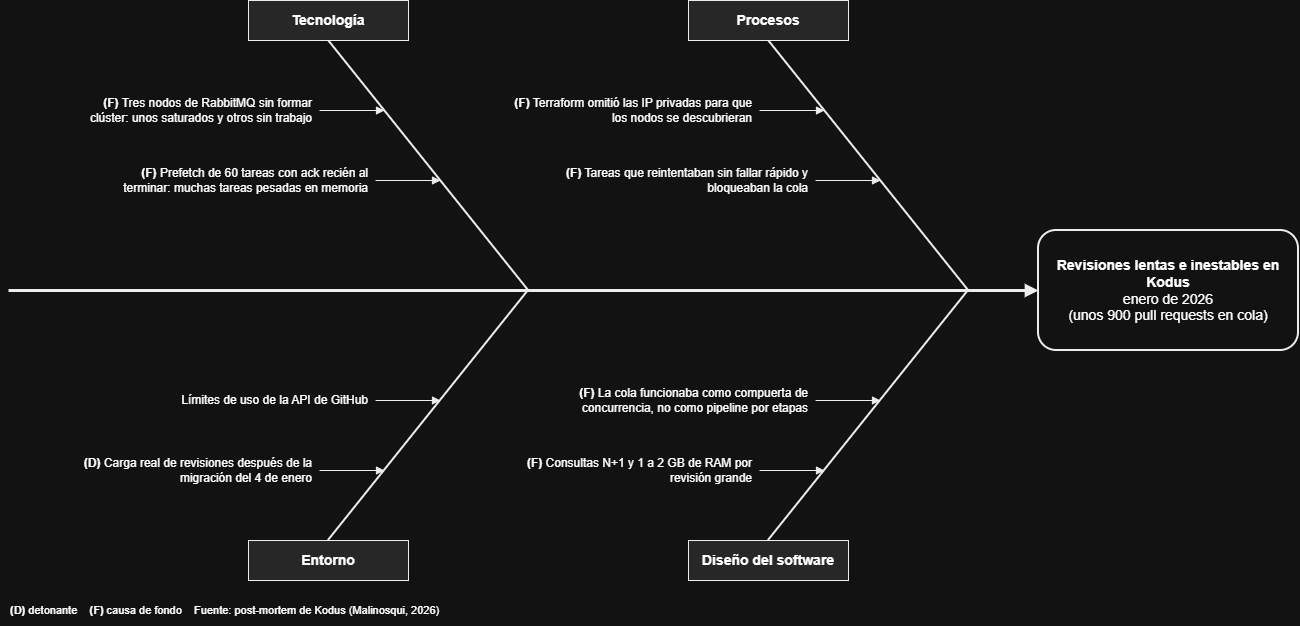
\includegraphics[width=\textwidth]{diagramas/causas.png}\\[0.2cm]
  {\small Detonante: la carga real después de la migración. Causa de fondo principal: RabbitMQ nunca funcionó como clúster \cite{malinosqui2026kodus}.}
\end{frame}

\begin{frame}{Cómo lo resolvieron}
  \begin{itemize}
    \item Corrigieron Terraform y los tres nodos formaron un solo clúster: la cola de 900 se vació en minutos.
    \item Bajaron el prefetch de 60 a 20 tareas por trabajador.
    \item Corrigieron las consultas N+1 y bajó el uso de memoria.
    \item Hicieron que las tareas trabadas pudieran salir de la cola.
  \end{itemize}
  \vspace{0.3cm}
  {\small Fuente: \cite{malinosqui2026kodus}}
\end{frame}
